\pagebreak 
\section{How to find out more about ECCO}
\centering
%\emph{\color{MidnightBlue} \Huge How to find out more about ECCO:}
\newp



\color{MidnightBlue}{A complete description of ECCO V4r4 together with all project documentation can be found at the
following web spaces:}
\par
\begin{longtable}{p{0.5\textwidth} p{0.45\textwidth}}

Main ECCO portal & \url{https://ecco-group.org/home.htm} \\ \hline \\
ECCO History & \url{https://ecco-group.org/about.htm} \\ \hline \\
ECCO data analysis tools & \url{https://ecco-group.org/analysis-tools.htm} \\ \hline \\
ECCO tutorial with Python language & \url{https://ecco-v4-python-tutorial.readthedocs.io/} \\ \hline \\
ECCO tutorial with Julia language & \url{https://ecco-group.org/storymaps.htm?id=69} \\ \hline \\
ECCO Tube (Images, Movies, StoryMaps and Brochures) & \url{https://ecco-group.org/media.htm} \\ \hline \\
ECCO Visualizations & \url{https://ecco-group.org/world-of-ecco.htm#series} \\ \hline \\
To contact ECCO team & \url{https://ecco-group.org/contact.htm}\\ \hline \\
\end{longtable}
\vspace{2.5cm}
%\color{blue}{
% 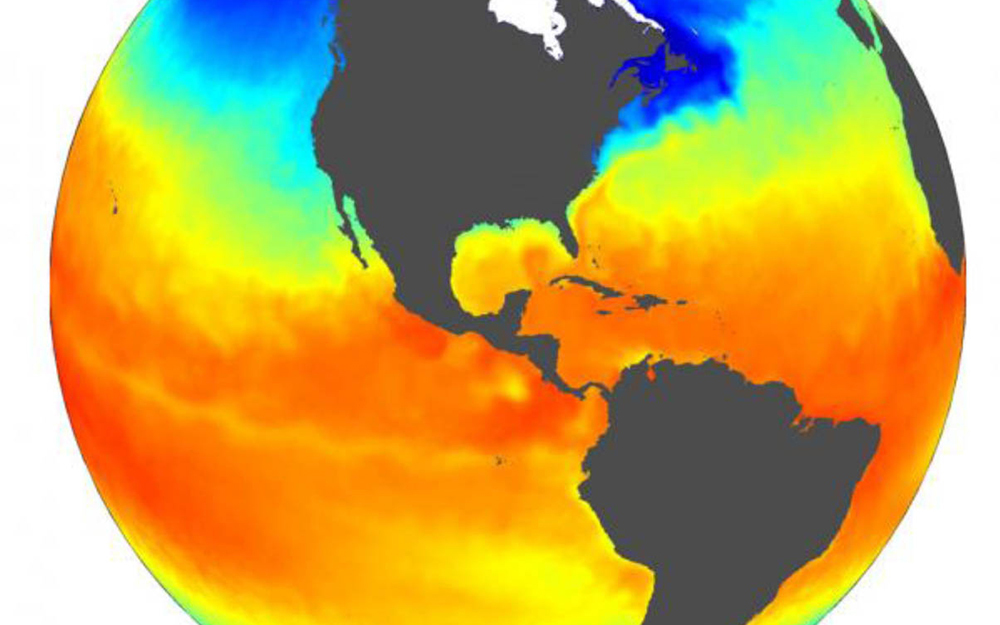
\includegraphics[width=0.4\textwidth]{../images/globe_1000px.jpeg}

\includegraphics[width=0.5\textwidth]{../images/ecco_logo_800_726.png}
% \newp

% \large{\color{MidnightBlue}\emph{GHRSST International Project Office}} \\
% \normalsize
% \color{MidnightBlue}NCEO, Department of Meteorology, \\
% University of Reading, \\
% United Kingdom
% \newp

% Tel +44 (0) 118 3785579 \\
% Fax +44 (0) 118 3785576 \\
% E-mail: \\
% \color{blue}{ghrsst-po@nceo.ac.uk}
% \color{MidnightBlue}

% \thispagestyle{empty}
% \vfill
% \footnotesize The GHRSST International Project Office is sponsored by the European Space Agency
% and the National Centre for Earth Observation, United Kingdom.